% ==============================================================================
% Fluxograma PRISMA 2020 (Page et al., 2021): identificação por bases de dados
% e registros. Preencher os valores de n. Incluído por \input no Capítulo 3.
% ==============================================================================
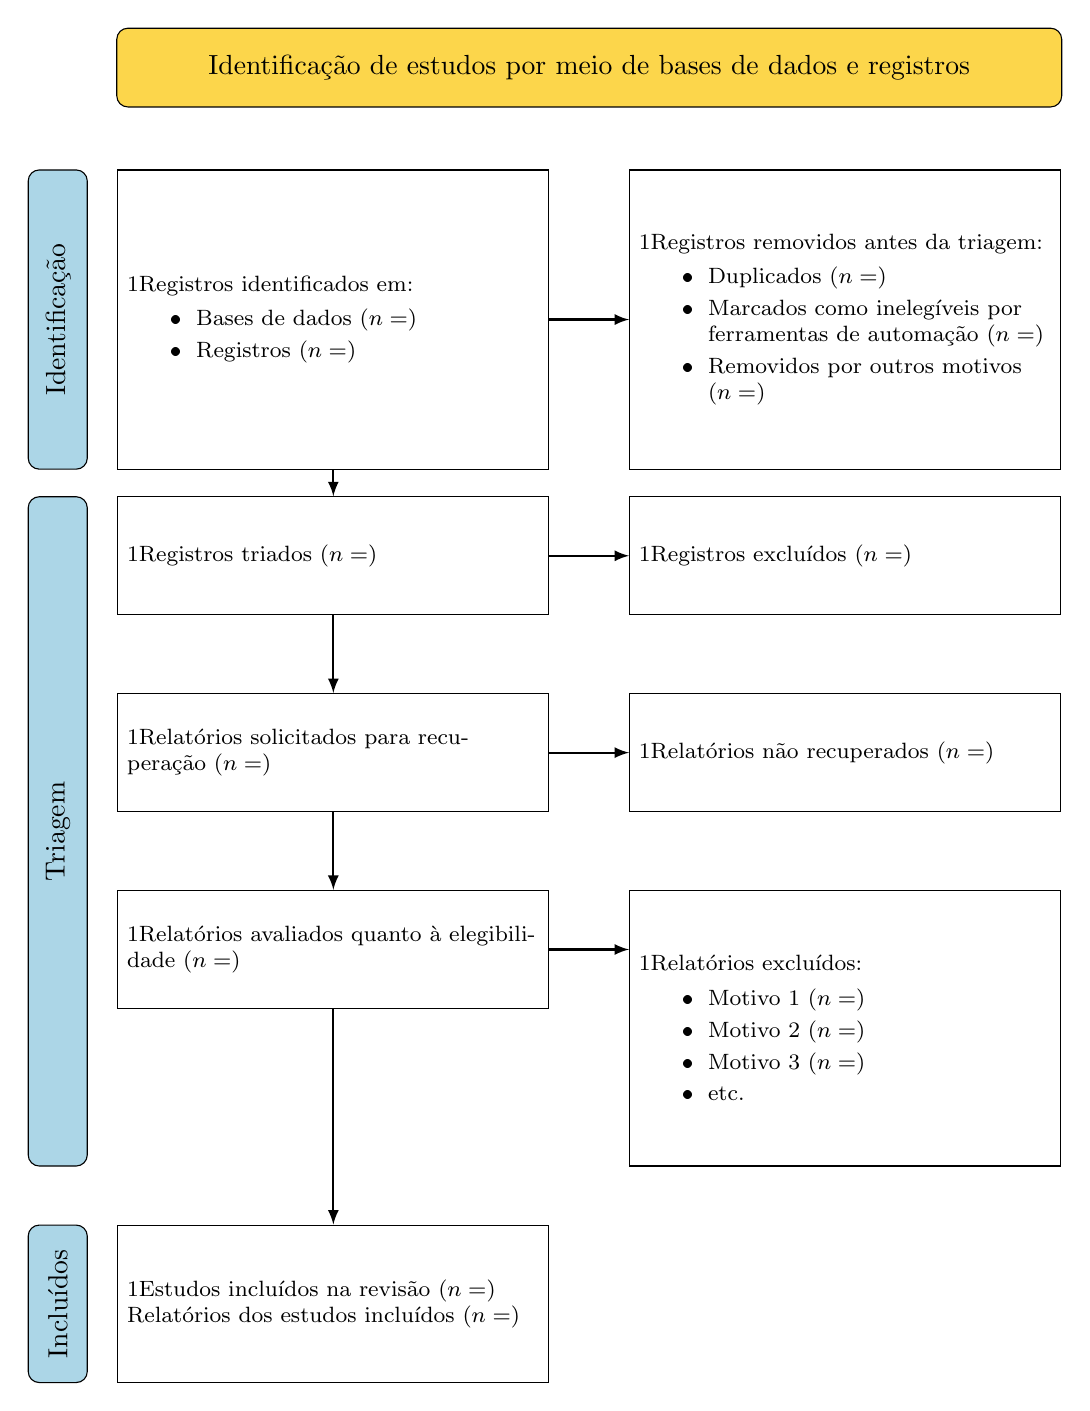
\begin{tikzpicture}[>=latex, font={\sffamily\small}]

    \tikzset{
      bluerect/.style={rectangle, rounded corners, minimum width=1.5cm, minimum height=0.75cm,
                       text centered, draw=black, fill=cyan!60!gray!45!white, rotate=90, font=\rmfamily},
      roundedrect/.style={rectangle, rounded corners, minimum width=12cm, minimum height=1cm,
                          text centered, draw=black, font=\rmfamily},
      textrect/.style={rectangle, minimum width=5.25cm, text width=5.24cm, minimum height=1cm,
                       draw=black, font={\rmfamily\footnotesize},
                       execute at begin node={\setstretch{1}\setlength{\itemsep}{0pt}}}
    }

    \node (top1) at (0, 11.2cm) [roundedrect, fill=yellow!80!red!70]
    {Identificação de estudos por meio de bases de dados e registros};

    \node (r1blue) at (-6.75cm, 8.0cm) [bluerect, minimum width=3.8cm]{Identificação};

    \node (r1left) at (-3.25cm, 8.0cm) [textrect, minimum height=3.8cm]
    {Registros identificados em:
        \begin{itemize}\setlength{\itemsep}{0pt}\setlength{\parsep}{0pt}\setlength{\topsep}{2pt}
            \item Bases de dados ($n=$)
            \item Registros ($n=$)
        \end{itemize}
    };

    \node (r1right) at (3.25cm, 8.0cm) [textrect, minimum height=3.8cm]
    {Registros removidos antes da triagem:
        \begin{itemize}\setlength{\itemsep}{0pt}\setlength{\parsep}{0pt}\setlength{\topsep}{2pt}
            \item Duplicados ($n=$)
            \item Marcados como inelegíveis por ferramentas de automação ($n=$)
            \item Removidos por outros motivos ($n=$)
        \end{itemize}
    };

    \node (r2blue) at (-6.75cm, 1.5cm) [bluerect, minimum width=8.5cm]{Triagem};

    \node (r2left) at (-3.25cm, 5.0cm) [textrect, minimum height=1.5cm]
    {Registros triados ($n=$)};

    \node (r2right) at (3.25cm, 5.0cm) [textrect, minimum height=1.5cm]
    {Registros excluídos ($n=$)};

    \node (r3left) at (-3.25cm, 2.5cm) [textrect, minimum height=1.5cm]
    {Relatórios solicitados para recuperação ($n=$)};

    \node (r3right) at (3.25cm, 2.5cm) [textrect, minimum height=1.5cm]
    {Relatórios não recuperados ($n=$)};

    \node (r4left) at (-3.25cm, 0cm) [textrect, minimum height=1.5cm]
    {Relatórios avaliados quanto à elegibilidade ($n=$)};

    \node (r4right) at (3.25cm, -1.0cm) [textrect, minimum height=3.5cm]
    {Relatórios excluídos:
        \begin{itemize}\setlength{\itemsep}{0pt}\setlength{\parsep}{0pt}\setlength{\topsep}{2pt}
            \item Motivo 1 ($n=$)
            \item Motivo 2 ($n=$)
            \item Motivo 3 ($n=$)
            \item etc.
        \end{itemize}
    };

    \node (r5blue) at (-6.75cm, -4.5cm) [bluerect, minimum width=2cm]{Incluídos};

    \node (r5left) at (-3.25cm, -4.5cm) [textrect, minimum height=2cm]
    {Estudos incluídos na revisão ($n=$)\\
     Relatórios dos estudos incluídos ($n=$)};

    % Conectores
    \draw[thick, ->] (r1left) -- (r1right);
    \draw[thick, ->] (r1left) -- (r2left);
    \draw[thick, ->] (r2left) -- (r2right);
    \draw[thick, ->] (r2left) -- (r3left);
    \draw[thick, ->] (r3left) -- (r3right);
    \draw[thick, ->] (r3left) -- (r4left);
    % Corrigido: no original, "-+ (0.5,0)" não alcançava a caixa de excluídos
    \draw[thick, ->] (r4left.east) -- (r4left.east -| r4right.west);
    \draw[thick, ->] (r4left) -- (r5left);

\end{tikzpicture}
